\documentclass[conference]{IEEEtran}
\IEEEoverridecommandlockouts
% The preceding line is only needed to identify funding in the first footnote. If that is unneeded, please comment it out.
\usepackage{cite}
\usepackage{amsmath,amssymb,amsfonts}
\usepackage{algorithmic}
\usepackage{graphicx}
\usepackage{textcomp}
\usepackage{xcolor}
\usepackage{hyperref}

\def\BibTeX{{\rm B\kern-.05em{\sc i\kern-.025em b}\kern-.08em
    T\kern-.1667em\lower.7ex\hbox{E}\kern-.125emX}}
\begin{document}

\title{Multi-Task Temporal and Spatial Networks for Precise Event Spotting in Volleyball Videos\\
\thanks{Identify applicable funding agency here. If none, delete this.}
}

\author{\IEEEauthorblockN{1\textsuperscript{st} Hoang Quoc Nguyen}
\IEEEauthorblockA{\textit{AI Robotics} \\
\textit{University of Science and Technology}\\
Daejeon, 34113, Republic of Korea \\
nqhoang@ust.ac.kr}
\and
\IEEEauthorblockN{2\textsuperscript{nd} Given Name Surname}
\IEEEauthorblockA{\textit{dept. name of organization (of Aff.)} \\
\textit{name of organization (of Aff.)}\\
City, Country \\
email address or ORCID}
\and
\IEEEauthorblockN{3\textsuperscript{rd} Given Name Surname}
\IEEEauthorblockA{\textit{dept. name of organization (of Aff.)} \\
\textit{name of organization (of Aff.)}\\
City, Country \\
email address or ORCID}
\and
\IEEEauthorblockN{4\textsuperscript{th} Given Name Surname}
\IEEEauthorblockA{\textit{dept. name of organization (of Aff.)} \\
\textit{name of organization (of Aff.)}\\
City, Country \\
email address or ORCID}
\and
\IEEEauthorblockN{5\textsuperscript{th} Given Name Surname}
\IEEEauthorblockA{\textit{dept. name of organization (of Aff.)} \\
\textit{name of organization (of Aff.)}\\
City, Country \\
email address or ORCID}
\and
\IEEEauthorblockN{6\textsuperscript{th} Given Name Surname}
\IEEEauthorblockA{\textit{dept. name of organization (of Aff.)} \\
\textit{name of organization (of Aff.)}\\
City, Country \\
email address or ORCID}
}

\maketitle

\begin{abstract}
    In sport videos analysis, especially in speedy sports such as Volleyball, understanding and localizing the precise timing and location of actions and events are critical. We introduce a new task: precise spatio-temporal event spotting, which aims to detect both when and where key events happen. To support this, we develop the KOVO Volleyball Event Dataset, featuring 947 rally videos, and 5,935 events, annotated for both temporal and spatial localization. Our best model achieves a combined mAP of 85.46 across various temporal and spatial thresholds. Notably, we find that incorporating spatial predictions enhances temporal mAP by 5.89 points, underscoring the synergy between spatial and temporal analysis. To the best of our knowledge, this is the first work addressing this task, establishing a strong baseline for future research in spatio-temporal event spotting.
\end{abstract}

\begin{IEEEkeywords}
precise event spotting, video understanding, spatial temporal event spotting, deep learning, volleyball, sport
\end{IEEEkeywords}

\section{Introduction}

Video understanding has emerged as a cornerstone in computer vision, offering valuable insights into dynamic scenes for applications such as sports analytics, surveillance, and autonomous systems. This field encompasses various tasks designed to interpret and analyze actions over time. Among these, \textit{Video Classification} aims to assign a single label to an entire video, providing a broad understanding of the content but often lacking frame-level precision. In contrast, \textit{Temporal Action Localization (TAL)} focuses on identifying time intervals where specific actions occur within untrimmed videos. Complementing these is \textit{Precise Action Spotting (PES)}, which identifies the precise frames that capture key events, requiring models to discern subtle temporal differences and distinguish visually similar frames \cite{spot22}.

Recent advancements in action spotting, such as \textit{T-DEED} \cite{tdeed23} and \textit{E2E-Spot} \cite{spot22}, have demonstrated the ability of models to achieve frame-level precision in fast-paced events using deep learning architectures. Datasets like \textit{FigureSkating} \cite{figureskating} and \textit{FineDiving} \cite{finediving} have been pivotal in advancing action spotting, emphasizing the importance of precise temporal detection in sports with individual athletes. However, these datasets are tailored to specific sports and do not capture the complexity and rapid dynamics of team-based, high-speed sports, such as volleyball.

In volleyball, rapid play transitions occur within specific areas of the court, making precise spatial localization as important as temporal accuracy. To address this, we introduce the new task of \textit{Precise spatio-temporal event spotting}, designed to detect both the exact timing and spatial location of key events. Unlike conventional action spotting, this task provides richer insights into player positioning and movement patterns, which are crucial for analyzing volleyball gameplay.

In other sports, datasets like \textit{SoccerNet-v2} \cite{soccernetv2} have pushed the boundaries of action spotting through rich temporal and spatial annotations, significantly advancing model capabilities. Yet, no equivalent dataset exists for volleyball, a sport characterized by its rapid exchanges and the need for precise localization of actions. To fill this gap, we introduce the \textit{KOVO Event Dataset}, comprising 947 rally videos, 890,797 frames, and 5,935 annotated key actions. This dataset offers granular annotations for both temporal and spatial event localization, making it a valuable resource for developing models that capture the intricacies of volleyball.

Our contributions are threefold:
\begin{itemize}
    \item \textbf{New Task Introduction:} We introduce the task of Precise spatio-temporal event spotting, specifically tailored for the dynamics of volleyball.
    \item \textbf{Dataset Development:} We present the \textit{KOVO Event Dataset}, the first of its kind to include detailed temporal and spatial annotations for volleyball rallies, aimed at fostering research in this area.
    \item \textbf{Model Development:} We propose a multi-task deep learning model that jointly predicts event timing and spatial positions, leveraging this dual focus to achieve improved performance. Notably, incorporating spatial predictions into our model enhances temporal mAP by 5.89 points.
\end{itemize}

Our best model achieves a temporal mAP of 90.59, a spatial mAP of 77.94, and a combined mAP of 85.46, providing a strong baseline for this new task. As far as we are aware, this work is the first to explore Precise spatio-temporal event spotting in volleyball, setting the stage for future research in this area.


% TODO: Fill this when finish paper
% The paper proceeds with a discussion of related work in Section 2, a detailed description of our approach in Section 3, the experimental setup in Section 4, results in Section 5, and conclusions in Section 6.


\section{Related work}

\subsection{Video Classification}

Video classification aims to predict a single label for an entire video, in contrast to event spotting, which requires precise frame-level labeling. This distinction introduces unique challenges: video classification can leverage sparse frame sampling \cite{tsn}, whereas event spotting demands dense sampling to capture rapid changes in events. Additionally, classification models often employ global space-time pooling \cite{8578773} or temporal consensus \cite{zhou2018temporalrelationalreasoningvideos} to produce video-level predictions, while event spotting necessitates preserving high temporal resolution.


\subsection{Temporal Action Localization}

The goal of Temporal Action Localization (TAL) is to localize the temporal intervals when specific actions occur in untrimmed videos, making it ideal for prolonged actions that are not instantaneous. In contrast to video classification, which assigns a single label to an entire video, TAL requires precise start and end times, adding more complexity.

Typically, there are two approaches to TAL: two-stage \cite{9578330,10.1007/978-3-319-46487-9_47} and one-stage \cite{10203543,zhang2022actionformer}. In two-stage models, action proposals are generated first then used for classification, while action class and temporal intervals are done in one streamlined process. Recently, advanced techniques such as Transformers and Feature Pyramid Network are incorporated to improve temporal precision across varying action duractions, like ActionFormer \cite{zhang2022actionformer} and TriDet \cite{tridet}. Anchor-free approaches \cite{9171561} have further enhanced flexibility in predicting actions without relying on predefined time windows.

Datasets and benchmarks such as ActivityNet \cite{ActivityNet}, EPIC-KITCHENS \cite{damen2018scalingegocentricvisionepickitchens}, and THUMOS Challenge \cite{Idrees_2017} have driven the development of TAL, which has become a central topic in Video Understand. By contrast, the precise identification of single-timestamp events remains less explored.

\subsection{Precise Event Spotting}

Precise Event Spotting (PES) aims to detect the exact frames of key events in untrimmed videos, making it ideal for fast, critical moments in sports. Unlike Temporal Action Localization (TAL), which spans broader time intervals, PES requires frame-level accuracy, crucial for detailed sports analysis where slight timing shifts can alter game interpretations.

Datasets like \textit{FigureSkating} \cite{figureskating} and \textit{FineDiving} \cite{finediving} have advanced PES with frame-level annotations, but focus on simpler, individual sports. Recent methods, such as \textit{T-DEED} \cite{tdeed23} and \textit{E2E-Spot} \cite{spot22}, enhance precision by refining temporal representations and avoiding pooling, but lack spatial context needed for team sports.

In volleyball, spatial localization is as critical as timing. Understanding event locations is key to analyzing player movements and strategies. Our work addresses this by introducing a new task and dataset for Precise spatio-temporal event spotting in volleyball, capturing both event timing and location.

Inspired by \textit{E2E-Spot} \cite{spot22}, our approach uses RegNet-Y \cite{radosavovic2020designingnetworkdesignspaces} with GSM \cite{9156729} for adaptive temporal shifts. This combination balances efficiency and precision, making it ideal for capturing complex spatio-temporal dynamics in volleyball.

\section{Dataset Overview}

\subsection{Data Content and Statistics}
\subsection{Annotation Process}
\subsection{Dataset Splits}
\subsection{Release and Access}
Given the large size of the dataset, we are unable to release the full-resolution (1280x720) videos in this paper. However, we have made a resized version (512x288 resolution) along with the corresponding annotations available on Kaggle, totaling 100GB. The dataset can be accessed at \url{www.kaggle.com/soon}.


\section{Proposed Method}
\subsection{Problem Formulation}
\textbf{Precise Spatio-Temporal Event Spotting (PSTES)} aims to identify both the precise time and location of events within untrimmed videos. For a sequence of \(N\) frames \(x_1, \ldots, x_N\) and a set of \(K\) event classes \(c_1, \ldots, c_K\), the goal is to predict a sparse set of frame indices where events occur, as well as the corresponding event class and spatial coordinates. Each prediction is represented as \((t, c_t, s_t)\), where \(t\) is the frame index, \(c_t\) is the predicted event class, and \(s_t\) is the spatial location of the event within that frame. A temporal prediction is deemed correct if it falls within a small temporal tolerance \(\sigma_f\) frames of the labeled event and matches the ground-truth class. Similarly, spatial predictions are deemed correct if the distance between the predicted location \(s_t\) and the ground-truth event location is within a specified threshold \(\sigma_p\). For PSTES, these tolerances are kept small, requiring precise frame-level accuracy, and it assumes that videos are captured with sufficiently high frame rates.

To achieve strong performance on this task, several important factors must be considered:

\begin{itemize}
    \item \textbf{Capturing Local Spatio-Temporal Features}: The model must be able to detect subtle visual changes and movements across adjacent frames, which is crucial for differentiating between events that may look quite similar.
    \item \textbf{Incorporating Long-Term Temporal Context}: By analyzing a wider temporal range, the model can better understand how events unfold over time, such as tracking how player movements or actions develop before and after a key moment.
    \item \textbf{Producing Dense Frame-Level Predictions}: For each frame \(x_t\), the model outputs predictions \((\hat{y}_t, \hat{s}_t)\), where \(\hat{y}_t \in \mathbb{R}^K\) represents the class probabilities in a vector of logits, and \(\hat{s}_t \in \mathbb{R}^2\) provides the spatial coordinates \((x, y)\) of the event in the frame. The event class \(c_t\) is determined by applying argmax to \(\hat{y}_t\), ensuring accuracy at the frame level for each event.
\end{itemize}

Meeting these requirements necessitates a robust, end-to-end architecture that effectively leverages both spatial and temporal data. Our approach employs a sequence model that integrates local spatio-temporal features to achieve this goal.


\subsection{Model Architecture}
To effectively learn spatio-temporal features, we propose a multi-task deep learning model comprising three key components: a Feature Extractor, a Dual-attention Feature Aggregation module, and Spatio-Temporal Prediction Heads. Drawing inspiration from Hong et al.\cite{spot22}, our model employs a RegNet-Y backbone \cite{radosavovic2020designingnetworkdesignspaces} with GSM \cite{9156729} for adaptive temporal shifts to extract features from each input frame. These features are subsequently aggregated via a dual-attention mechanism, integrating spatial and temporal information to enhance feature representations. The model then predicts event classes and spatial coordinates through distinct heads, each optimized with a multi-task loss function that balances temporal and spatial prediction objectives.

\begin{figure}[htbp]
    \centerline{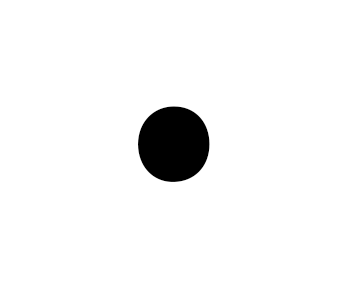
\includegraphics{fig1.png}}
    \caption{Example of a figure caption.}
    \label{fig}
    \end{figure}
\subsubsection{Feature Extractor}
The Feature Extractor processes each frame \( x_t \in \mathbb{R}^{H \times W \times 3} \) using a RegNet-Y backbone combined directly with a Gate Shift Module (GSM) to capture spatial and temporal information simultaneously. By embedding GSM within RegNet-Y, the network learns not only spatial structures but also the temporal motion present across frames, as GSM shifts features adaptively to track long-term dependencies. This integration produces a spatio-temporal feature \( f_t \in \mathbb{R}^d \) that captures both motion and spatial details, equipping the model to accurately interpret the flow of events and predict their progression.



\subsubsection{Dual-attention Feature Aggregation}
\begin{itemize}
    % TODO: Review the original Squeeze and Excitation paper, to check if the explanation is correct. Also, add citation
    \item \textbf{Channel Attention Module:} The Channel Attention Module employs a Squeeze-and-Excitation mechanism to refine feature representation by emphasizing informative channels. This allows the model to focus on key spatial features within each frame, enhancing its sensitivity to subtle visual cues and spatial patterns. By directing attention to relevant regions, the module aids the model in distinguishing between visually similar events occurring in different locations, improving accuracy in event differentiation.

    % TODO: Review the original Transformer paper, to check if the explanation is correct. Also, add citation
    \item \textbf{Temporal Attention Module:} Utilizing multi-head attention as described in the *Attention is All You Need* paper, the Temporal Attention Module aggregates features across adjacent frames to capture long-term dependencies and evolving event dynamics. By focusing on relevant temporal patterns within a broader context, this module enables the model to anticipate the timing and progression of key events with greater accuracy.

\end{itemize}
\subsubsection{Spatio-Temporal Prediction Heads}
The model predicts event classes and spatial coordinates through distinct heads, each optimized with a multi-task loss function that balances temporal and spatial prediction objectives. The event class head outputs a vector of logits \(\hat{y}_t\) representing the predicted class probabilities for each event, while the spatial head outputs a vector of coordinates \(\hat{s}_t\) representing the predicted spatial location of the event within the frame. By jointly optimizing these heads, the model can effectively learn spatio-temporal features and produce accurate predictions for both event timing and location.
\subsubsection{Multi-task Loss Function}
The model is trained with a multi-task loss function that balances temporal and spatial prediction objectives, ensuring that the model learns to predict both when and where key events occur. The loss function is defined as the sum of two terms: a temporal classification loss and a spatial regression loss. The temporal classification loss penalizes errors in event class predictions


\section{Experiments}
\subsection{Implementation Details}
\subsection{Training Strategy}
\subsection{Evaluation Metrics}

\section{CONCLUSIONS}
\section*{Acknowledgment}

\bibliographystyle{IEEEtran}
\bibliography{references}
\end{document}
